\section{Analisi dei Dati}
La prima analisi effettuata sui dati ricavati dall'elaborazione dei risultati ottenuti da \textbf{Nicad} e \textbf{SonarQube} ha riguardato il numero di cloni sulle $4$ versioni per ogni progetto. I risultati hanno evidenziato che al crescere della versione la presenza di cloni aumenta, in particolare:
\begin{itemize}
	\item in \textbf{DnsJava}, come mostrato in \autoref{fig:nCloniDnsJava}, si hanno $146$ cloni nelle versioni $2.1.5$ e $2.1.6$, $147$ nella versione $2.1.7$ e $151$ nella $2.1.8$;
	\item in \textbf{Jabref}, come mostrato in \autoref{fig:nCloniJabRef}, si hanno $336$ nella versione $4.0$, $353$ nella $4.1$, $228$ nella $4.2$ e $357$ nella versione $4.3$;
	\item in \textbf{Fastjson}, come mostrato in \autoref{fig:nCloniFastjson}, si hanno $1107$ cloni nella versione $1.2.20$, $1230$ nella $1.2.30$ , $1292$ nella $1.2.40$ e $1358$ nella $1.2.50$.
\end{itemize}
\begin{figure}[h]
	\centering
	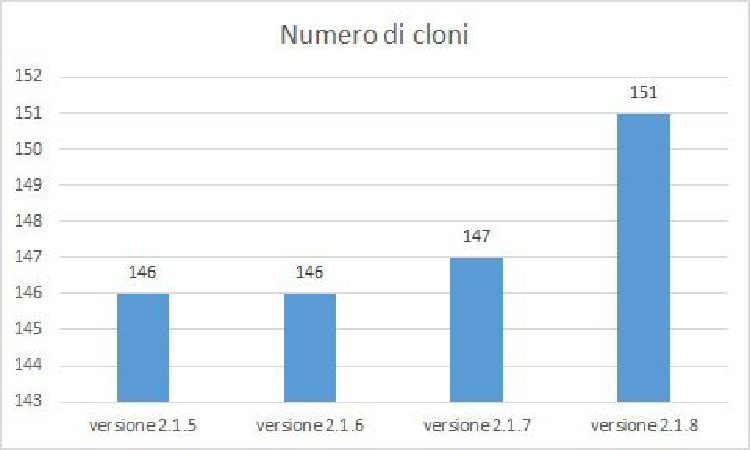
\includegraphics[scale=0.7, trim = 0cm 0cm 0cm 0cm, clip=true]{Grafici_dnsJava/NumeroCloni.pdf}
	\caption{Analisi numero cloni DnsJava}
	\label{fig:nCloniDnsJava}
\end{figure}
\begin{figure}[h]
	\centering
	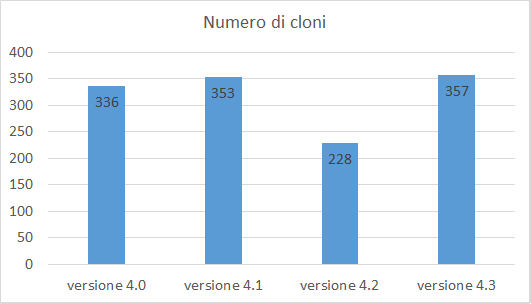
\includegraphics[scale=0.58, trim = 0cm 0cm 0cm 0cm, clip=true]{Grafici_jabRef/NumeroCloni.png}
	\caption{Analisi numero cloni JabRef}
	\label{fig:nCloniJabRef}
\end{figure}
\begin{figure}[h]
	\centering
	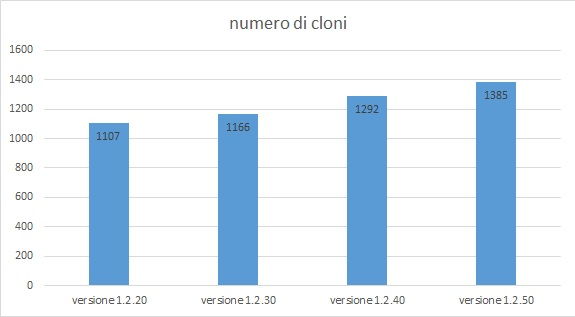
\includegraphics[scale=0.7, trim = 0cm 0cm 0cm 0cm, clip=true]{Grafici_fastJson/NumeroCloni.jpg}
	\caption{Analisi numero cloni FastJson}
	\label{fig:nCloniFastjson}
\end{figure}
Si nota dunque che l'unico dato anomalo si ha sulla versione $4.2$ di JabRef in cui il numero di cloni diminuisce rispetto alla versione precedente. Questo risultato non va però ad inficiare il trend verificato nelle analisi degli altri progetti in quanto si nota che nella versione $4.3$ vi è, non solo un aumento rispetto alla versione $4.2$, ma addirittura un incremento rispetto a tutte le precedenti versioni. 

La seconda analisi ha riguardato il \textbf{numero di cloni di ogni tipo} per le $4$ versioni di ciascuno dei progetti presi in considerazione. In linea di massima il numero di cloni di tipo $3$ è sempre maggiore rispetto ai cloni di tipo $1$ e $2$. In particolare:
\begin{itemize}
	\item in \textbf{DnsJava}, come mostrato in \autoref{fig:tipiCloniDnsJava}, si hanno:
		\begin{itemize}
				\item versione $2.1.5$: 7 cloni di tipo 1, 27 cloni di tipo 2, 112 di tipo 3;
				\item versione $2.1.6$: 7 cloni di tipo 1, 27 cloni di tipo 2, 112 di tipo 3;
				\item versione $2.1.7$: 7 cloni di tipo 1, 27 cloni di tipo 2, 113 di tipo 3;
				\item versione $2.1.8$: 9 cloni di tipo 1, 27 cloni di tipo 2, 115 di tipo 3;		
		\end{itemize}
	\item in \textbf{JabRef}, come mostrato in \autoref{fig:tipiCloniJabRef}, si hanno:
				\begin{itemize}
			\item versione $4.0$: 8 cloni di tipo 1, 48 cloni di tipo 2,280 di tipo 3;
			\item versione $4.1$: 10 cloni di tipo 1, 49 cloni di tipo 2, 294 di tipo 3;
			\item versione $4.2$: 2 cloni di tipo 1, 20 cloni di tipo 2, 206 di tipo 3;
			\item versione $4.3$: 8 cloni di tipo 1, 49 cloni di tipo 2, 300 di tipo 3;		
		\end{itemize}
	\item in \textbf{FastJson}, come mostrato in \autoref{fig:tipiCloniFastjson}, si hanno:
	\begin{itemize}
		\item versione $1.2.20$: 270 cloni di tipo 1, 120 cloni di tipo 2,717 di tipo 3;
		\item versione $1.2.30$: 284 cloni di tipo 1, 140 cloni di tipo 2, 742 di tipo 3;
		\item versione $1.2.40$: 301 cloni di tipo 1, 150 cloni di tipo 2, 841 di tipo 3;
		\item versione $1.2.50$: 313 cloni di tipo 1,154 cloni di tipo 2, 918 di tipo 3;		
	\end{itemize}
\end{itemize}
Quello che si nota è che in tutti i progetti analizzati il numero di cloni di tipo 3 è predominante. I cloni di tipo 2 sono maggiori rispetto a quelli di tipo 1 tranne che in \textbf{FastJson} essendo quest'ultima una libreria.
\begin{figure}[h]
	\centering
	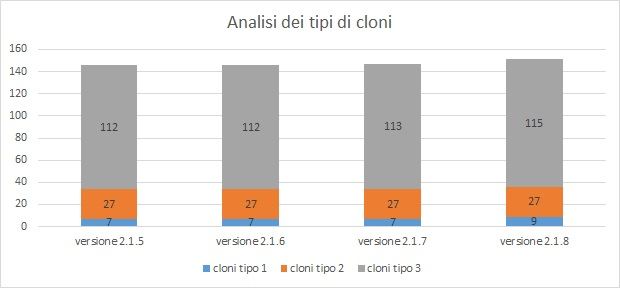
\includegraphics[scale=0.7, trim = 0cm 0cm 0cm 0cm, clip=true]{Grafici_dnsJava/TipiCloni.jpg}
	\caption{Analisi tipo cloni DnsJava}
	\label{fig:tipiCloniDnsJava}	
\end{figure}
\begin{figure}[h]
	\centering
	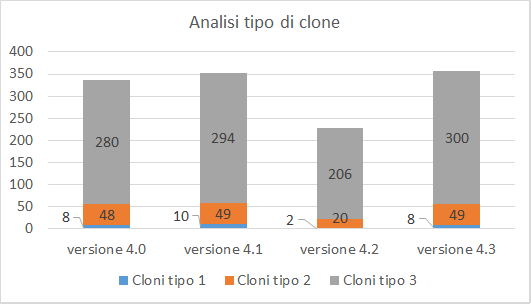
\includegraphics[scale=0.7, trim = 0cm 0cm 0cm 0cm, clip=true]{Grafici_jabRef/TipiCloni.png}
	\caption{Analisi tipo cloni JabRef}
	\label{fig:tipiCloniJabRef}
\end{figure}
\begin{figure}[h]
	\centering
	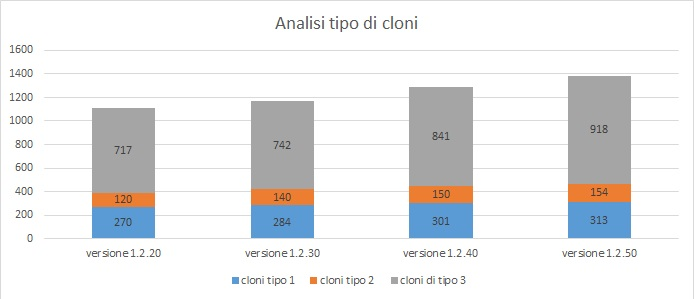
\includegraphics[scale=0.58, trim = 0cm 0cm 0cm 0cm, clip=true]{Grafici_fastJson/TipiCloni.jpg}
	\caption{Analisi tipo cloni FastJson}
	\label{fig:tipiCloniFastjson}
\end{figure}
Procedendo nell'analisi è stato individuato il numero di file con e senza cloni:
\begin{itemize}
	\item in \textbf{DnsJava}, come mostrato in \autoref{fig:percentualeDnsJava} si hanno:
	\begin{itemize}
		\item nella versione 2.1.5 60 file con cloni e 129 senza cloni;
		\item nella versione 2.1.6 60 file con cloni e 130 senza cloni;
		\item nella versione 2.1.7 61 file con cloni e 134 senza cloni;
		\item nella versione 2.1.8 65 file con cloni e 131 senza cloni;
	\end{itemize}
	\item in \textbf{JabRef}, come mostrato in \autoref{fig:percentualeJabRef}, si hanno:
	\begin{itemize}
		\item nella versione 4.0 156 file con cloni e 1373 senza cloni;
		\item nella versione 4.1 158 file con cloni e 1409 senza cloni;
		\item nella versione 4.2 76 file con cloni e 1618 senza cloni;
		\item nella versione 4.3 160 file con cloni e 1542 senza cloni;
	\end{itemize}
		\item in \textbf{FastJson}, come mostrato in \autoref{fig:percentualeFastjson}, si hanno:
	\begin{itemize}
		\item nella versione 1.2.20 480 file con cloni e 1473 senza cloni;
		\item nella versione 1.2.30 510 file con cloni e 1639 senza cloni;
		\item nella versione 1.2.40 576 file con cloni e 1908 senza cloni;
		\item nella versione 1.2.50 598 file con cloni e 2047 senza cloni;
	\end{itemize}
\end{itemize}
AGGIUNGI CONSIDERAZIONE SU PERCENTUALE
\begin{figure}[h]
	\centering
	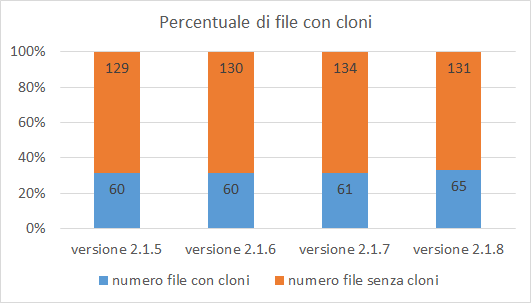
\includegraphics[scale=0.3, trim = 0cm 0cm 0cm 0cm, clip=true]{Grafici_dnsJava/PercentualeFileCloni.png}
	\caption{Analisi percentuale file con e senza cloni DnsJava}
	\label{fig:percentualeDnsJava}	
\end{figure}
\begin{figure}[h]
	\centering
	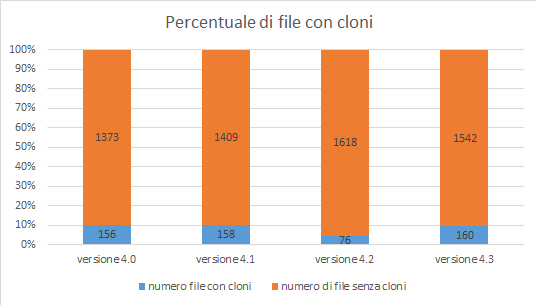
\includegraphics[scale=0.7, trim = 0cm 0cm 0cm 0cm, clip=true]{Grafici_jabRef/PercentualeFileCloni.png}
	\caption{Analisi percentuale file con e senza cloni JabRef}
	\label{fig:percentualeJabRef}
\end{figure}
\begin{figure}[h]
	\centering
	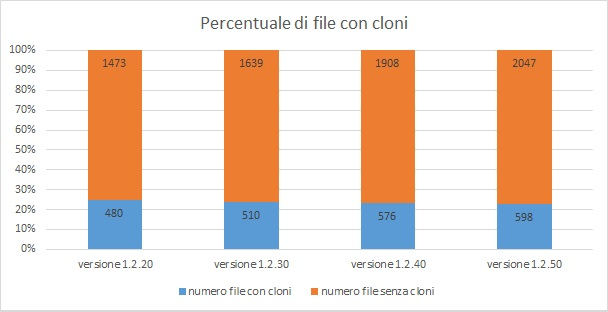
\includegraphics[scale=0.7, trim = 0cm 0cm 0cm 0cm, clip=true]{Grafici_fastJson/PercentualeFileConCloni.jpg}
	\caption{Analisi percentuale file con e senza cloni FastJson}
	\label{fig:percentualeFastjson}
\end{figure}
Si è proceduto all'analisi della presenza di code smell nei file con e senza cloni considerando i valori medi. Si è visto che nei file contenenti cloni, il numero medio di code smell è in generale maggiore rispetto al caso in cui il file non contiene i cloni stessi. In particolare:
\begin{itemize}
	\item in DnsJava, come mostrato in \autoref{fig:codeSmellDnsJava}:
	\begin{itemize}
		\item nella versione 2.1.5 in media, il numero di code smell è 63 nei file senza cloni e 209 in quelli con i cloni;
		\item nella versione 2.1.6 in media, il numero di code smell è 63 nei file senza cloni e 213 in quelli con i cloni;
		\item nella versione 2.1.7 in media, il numero di code smell è 61 nei file senza cloni e 220 in quelli con i cloni;
		\item nella versione 2.1.8 in media, il numero di code smell è 61 nei file senza cloni e 219 in quelli con i cloni;
	\end{itemize}
	\item in JabRef, come mostrato in \autoref{fig:codeSmellJabRef}:
	\begin{itemize}
		\item nella versione 4.0 in media, il numero di code smell è 36 nei file senza cloni e 156 in quelli con i cloni;
		\item nella versione 4.1 in media, il numero di code smell è 41 nei file senza cloni e 148 in quelli con i cloni;
		\item nella versione 4.2 in media, il numero di code smell è 38 nei file senza cloni e 155 in quelli con i cloni;
		\item nella versione 4.3 in media, il numero di code smell è 38 nei file senza cloni e 88 in quelli con i cloni;
	\end{itemize}
	\item in FastJson, come mostrato in \autoref{fig:codeSmellFastjson}:
	\begin{itemize}
		\item nella versione 1.2.20 in media, il numero di code smell è 30 nei file senza cloni e 125 in quelli con i cloni;
		\item nella versione 1.2.30 in media, il numero di code smell è 28 nei file senza cloni e 138 in quelli con i cloni;
		\item nella versione 1.2.40 in media, il numero di code smell è 28 nei file senza cloni e 177 in quelli con i cloni;
		\item nella versione 1.2.50 in media, il numero di code smell è 30 nei file senza cloni e 184 in quelli con i cloni;
	\end{itemize}
\end{itemize}
La differenza risulta maggiormente evidente in \textbf{FastJson}.
\begin{figure}[h]
	\centering
	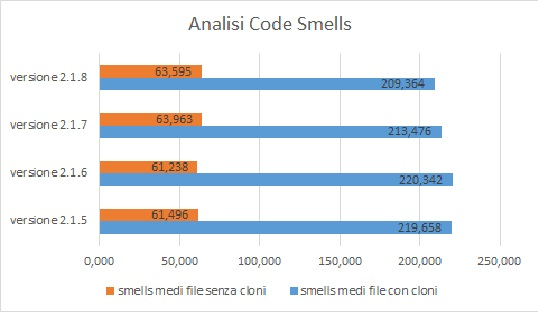
\includegraphics[scale=0.7, trim = 0cm 0cm 0cm 0cm, clip=true]{Grafici_dnsJava/CodeSmells.jpg}
	\caption{Numero medio code smell file con e senza cloni DnsJava}
	\label{fig:codeSmellDnsJava}	
\end{figure}
\begin{figure}[h]
	\centering
	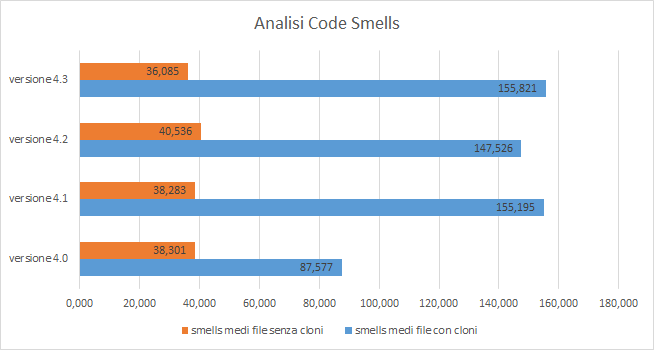
\includegraphics[scale=0.7, trim = 0cm 0cm 0cm 0cm, clip=true]{Grafici_jabRef/CodeSmells.png}
	\caption{Numero medio code smell file con e senza cloni JabRef}
	\label{fig:codeSmellJabRef}
\end{figure}
\begin{figure}[h]
	\centering
	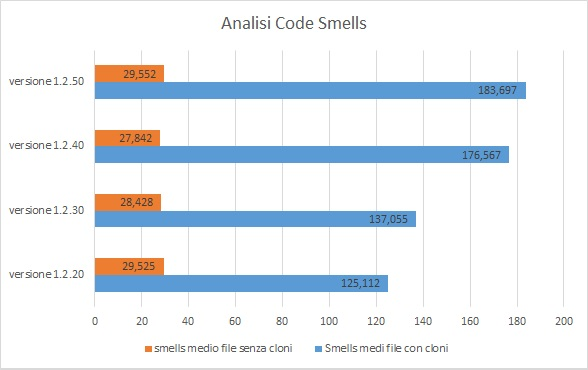
\includegraphics[scale=0.7, trim = 0cm 0cm 0cm 0cm, clip=true]{Grafici_fastJson/CodeSmell.jpg}
	\caption{Numero medio code smell file con e senza cloni FastJson}
	\label{fig:codeSmellFastjson}
\end{figure}
La stessa analisi è stata effettuata prendendo in considerazione il technical debt. In particolare sono stati ottenuti i seguenti risultati:
\begin{itemize}
		\item in DnsJava, come mostrato in \autoref{fig:tdDnsJava}:
	\begin{itemize}
		\item nella versione 2.1.5 in media, il techical debt è di 319 minuti nei file senza cloni e 1240 minuti in quelli con i cloni;
		\item nella versione 2.1.6 in media, il techical debt è di è 321 minuti nei file senza cloni e 1267 in quelli con i cloni;
		\item nella versione 2.1.7 in media, il techical debt è di 291 minuti nei file senza cloni e 1330 minuti in quelli con i cloni;
		\item nella versione 2.1.8 in media, il techical debt è di 292 nei file senza cloni e 1327 in quelli con i cloni;
	\end{itemize}
	\item in JabRef, come mostrato in \autoref{fig:tdJabRef}:
	\begin{itemize}
		\item nella versione 4.0 in media, il techical debt è di 177 minuti nei file senza cloni e 1104 minuti in quelli con i cloni;
		\item nella versione 4.1 in media, il techical debt è di 177 minuti nei file senza cloni e 1109 minuti in quelli con i cloni;
		\item nella versione 4.2 in media, il techical debt è di 185 minuti nei file senza cloni e 1232 in quelli con i cloni;
		\item nella versione 4.3 in media, il techical debt è di 163 nei file senza cloni e 1090 in quelli con i cloni;
	\end{itemize} 
		\item in FastJson, come mostrato in \autoref{fig:tdFastjson}:
	\begin{itemize}
		\item nella versione 1.2.20 in media, il techical debt è di 130 minuti nei file senza cloni e 655 in quelli con i cloni;
		\item nella versione 1.2.30 in media, il techical debt è di 124 minuti nei file senza cloni e 727 minuti in quelli con i cloni;
		\item nella versione 1.2.40 in media, il techical debt è di 122 minuti nei file senza cloni e 1047 in quelli con i cloni;
		\item nella versione 1.2.50 in media, il techical debt è di 125 minuti nei file senza cloni e 1143 in quelli con i cloni;
	\end{itemize}
\end{itemize}
Si nota quindi che il tempo necessario per gestire e quindi manutenere una classe in cui sono presenti dei cloni è più alto rispetto al caso in cui nella classe non risultano presenti i cloni stessi. Al fine di validare tale risultato, è stata effettuata un'analisi ulteriore. In particolare, per ogni versione di ogni progetto è stato considerato il rapporto tra code smell e techical debt. I risultati ottenuti sono i seguenti:
%%%ANALISI RAPPORTO%%%%
\begin{itemize}
	\item in DnsJava, come mostrato in \autoref{fig:rapDnsJava}, il rapporto tra technical debt e code smell è pari a circa 4 minuti nel caso di file senza cloni e a 5 nel caso di file con cloni in tutte e tre le versioni;
	\item in JabRef, come mostrato in \autoref{fig:rapJabRef}, il rapporto risulta circa pari a 4 nel caso di file senza cloni in tutte e tre le versioni. Nel caso di file con cloni
	\item in FastJson, come mostrato in \autoref{fig:tdFastjson}:
	\begin{itemize}
		\item nella versione 1.2.20 in media, il techical debt è di 130 minuti nei file senza cloni e 655 in quelli con i cloni;
		\item nella versione 1.2.30 in media, il techical debt è di 124 minuti nei file senza cloni e 727 minuti in quelli con i cloni;
		\item nella versione 1.2.40 in media, il techical debt è di 122 minuti nei file senza cloni e 1047 in quelli con i cloni;
		\item nella versione 1.2.50 in media, il techical debt è di 125 minuti nei file senza cloni e 1143 in quelli con i cloni;
	\end{itemize}
\end{itemize}

\begin{figure}[h]
	\centering
	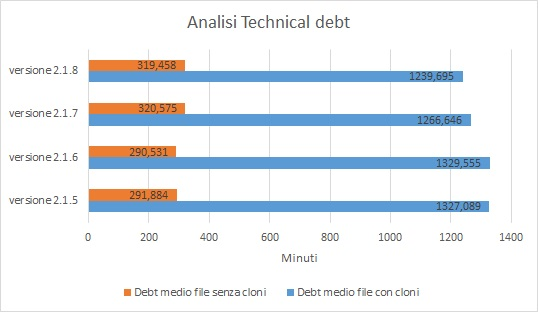
\includegraphics[scale=0.7, trim = 0cm 0cm 0cm 0cm, clip=true]{Grafici_dnsJava/TechnicalDebt.jpg}
	\caption{Techical Debt medio file con e senza cloni DnsJava}
	\label{fig:tdDnsJava}	
\end{figure}
\begin{figure}[h]
	\centering
	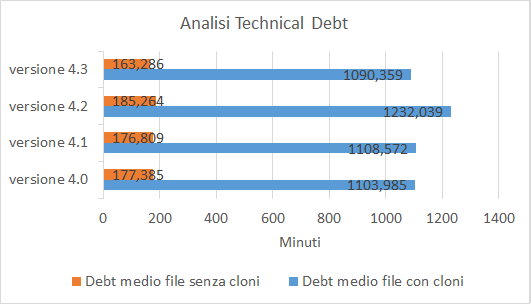
\includegraphics[scale=0.7, trim = 0cm 0cm 0cm 0cm, clip=true]{Grafici_jabRef/TechnicalDebt.png}
	\caption{Techical Debt medio file con e senza cloni JabRef}
	\label{fig:tdJabRef}
\end{figure}
\begin{figure}[h]
	\centering
	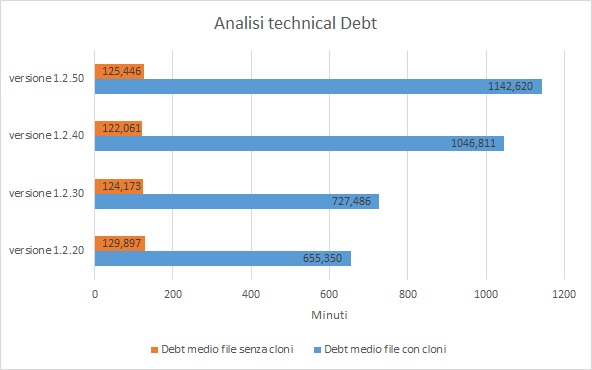
\includegraphics[scale=0.7, trim = 0cm 0cm 0cm 0cm, clip=true]{Grafici_fastJson/TechnicalDebt.jpg}
	\caption{Techical Debt medio file con e senza cloni FastJson}
	\label{fig:tdFastjson}
\end{figure}

%%%%%%%%%%%%%%%%%%%%%%%%%%%%%%%%%%%
\begin{figure}[h]
	\centering
	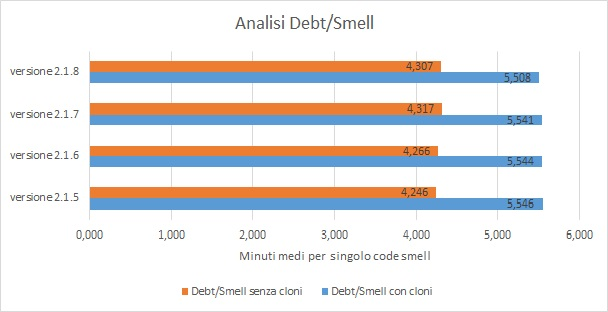
\includegraphics[scale=0.7, trim = 0cm 0cm 0cm 0cm, clip=true]{Grafici_dnsJava/Debt-Smells.jpg}
	\caption{Rapporto $\frac{code smell}{technical debt}$ file con e senza cloni DnsJava}
	\label{fig:rapDnsJava}	
\end{figure}
\begin{figure}[h]
	\centering
	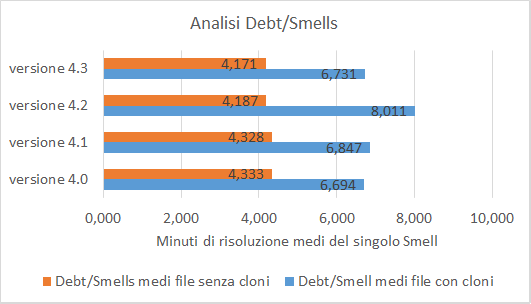
\includegraphics[scale=0.7, trim = 0cm 0cm 0cm 0cm, clip=true]{Grafici_jabRef/Debt-Smells.png}
	\caption{Rapporto $\frac{code smell}{technical debt}$ file con e senza cloni JabRef}
	\label{fig:rapJabRef}
\end{figure}
\begin{figure}[h]
	\centering
	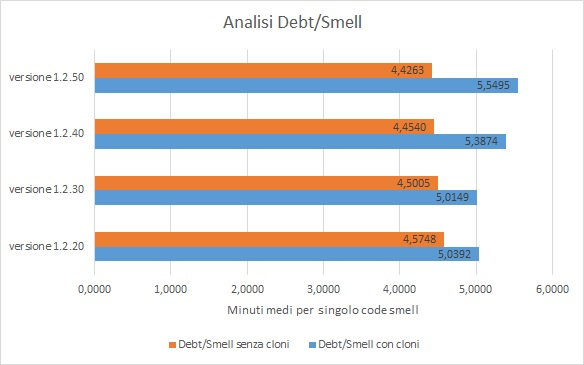
\includegraphics[scale=0.7, trim = 0cm 0cm 0cm 0cm, clip=true]{Grafici_fastJson/Debt-Smell.jpg}
	\caption{Rapporto $\frac{code smell}{technical debt}$ file con e senza cloni FastJson}
	\label{fig:rapFastjson}
\end{figure}
